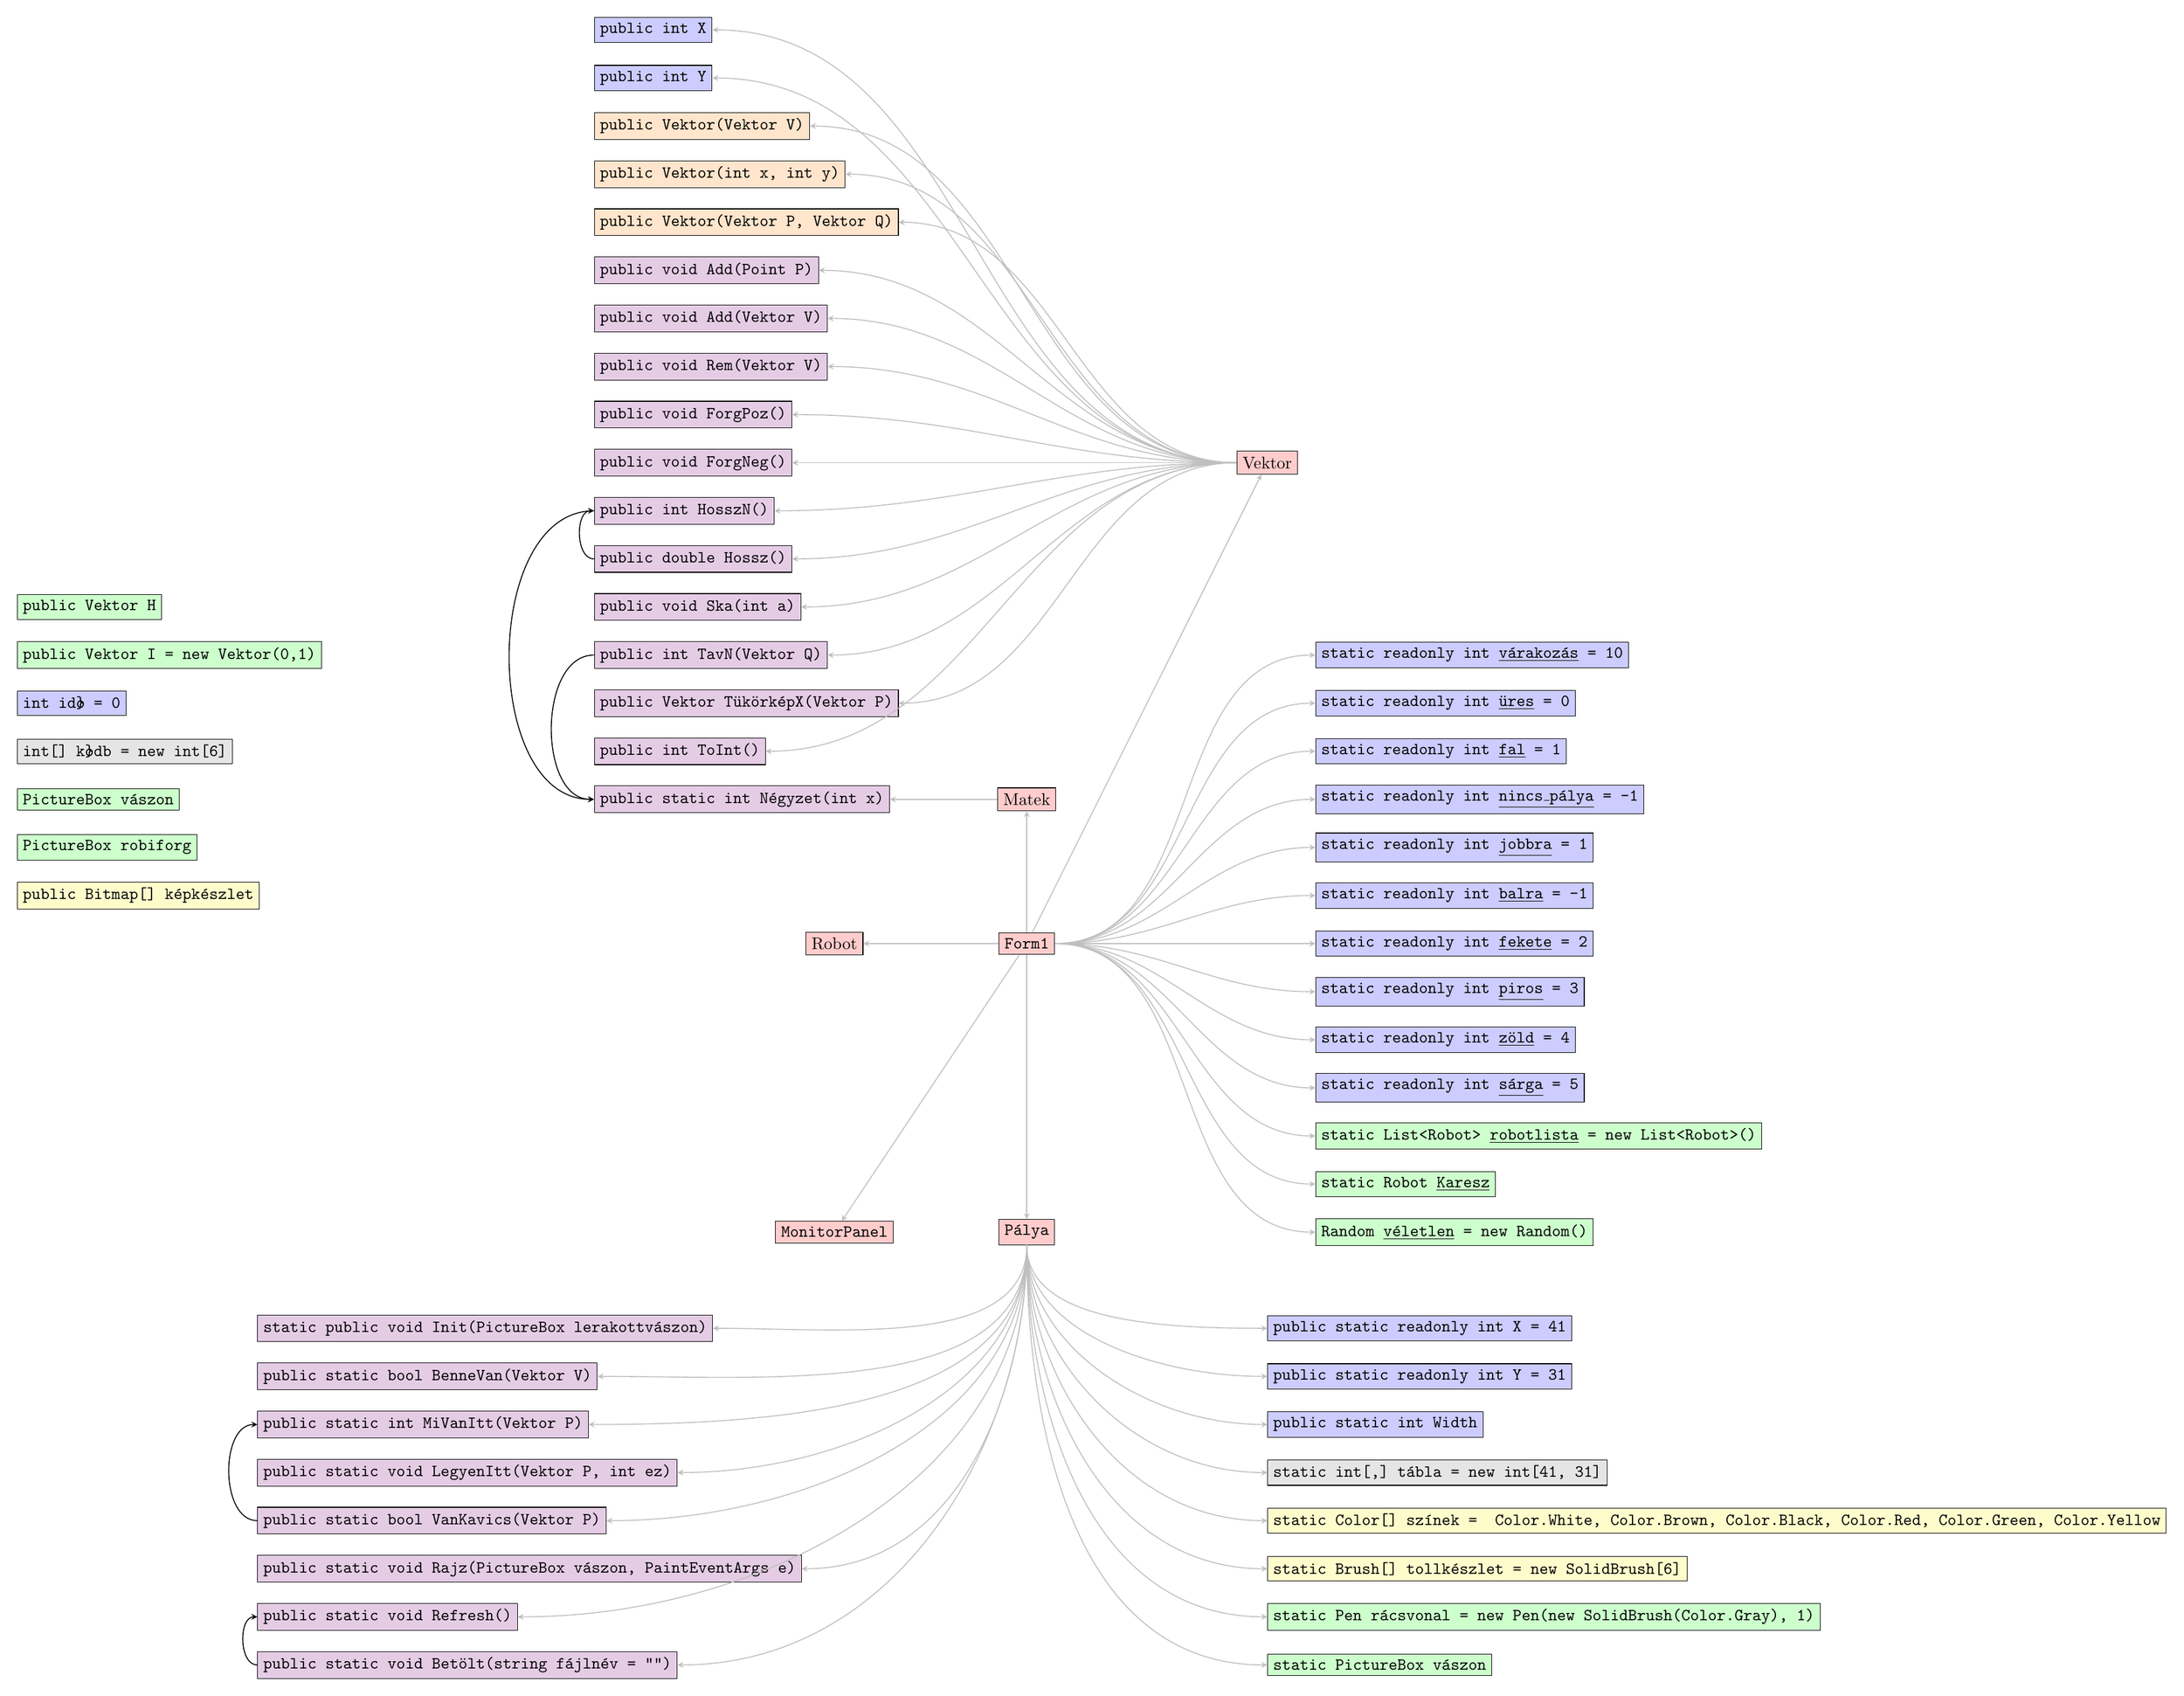
\begin{tikzpicture}[yscale=-1, 
valtozo/.style={anchor=west, rectangle,draw,fill=blue!20},
objektum/.style={anchor=west, rectangle,draw,fill=green!20},
class/.style={rectangle,draw,fill=red!20},
valtozohalmaz/.style={anchor=west,rectangle,draw,fill=gray!20},
objektumhalmaz/.style={anchor=west,rectangle,draw,fill=yellow!20},
method/.style={anchor=west,rectangle,draw,fill=violet!20},
konstruktor/.style={anchor=west,rectangle,draw,fill=orange!20},
meghivja/.style={->, line width=.2mm, >=stealth},
gyereke/.style={->, line width=.2mm, >=stealth, gray!50}
]

\node[class] (Form1) at (0,0) {\tt Form1};

\node[valtozo] (varakozas) at (6,-6) {\tt static readonly int \underline{várakozás} = 10};
\node[valtozo] (ures) at (6,-5) {\tt static readonly int \underline{üres} = 0};
\node[valtozo] (fal) at (6,-4) {\tt static readonly int \underline{fal} = 1};
\node[valtozo] (nincspalya) at (6,-3) {\tt static readonly int \underline{nincs\_pálya} = -1};
\node[valtozo] (jobbra) at (6,-2) {\tt static readonly int \underline{jobbra} = 1};
\node[valtozo] (balra) at (6,-1) {\tt static readonly int \underline{balra} = -1};
\node[valtozo] (fekete) at (6,0) {\tt static readonly int \underline{fekete} = 2};
\node[valtozo] (piros) at (6,1) {\tt static readonly int \underline{piros} = 3};
\node[valtozo] (zold) at (6,2) {\tt static readonly int \underline{zöld} = 4};
\node[valtozo] (sarga) at (6,3) {\tt static readonly int \underline{sárga} = 5};
\node[objektum] (robotlista) at (6,4) {\tt static List<Robot> \underline{robotlista} = new List<Robot>()};
\node[objektum] (Karesz) at (6,5) {\tt static Robot \underline{Karesz}};
\node[objektum] (veletlen) at (6,6) {\tt Random \underline{véletlen} = new Random()};

\foreach \n in {varakozas,ures,fal,nincspalya,jobbra,balra,fekete,piros,zold,sarga,robotlista,Karesz,veletlen}
{\draw[gyereke](Form1)edge[in = 180, out=0](\n);}

\node[class] (MonitorPanel) at (-4,6) {\tt MonitorPanel};
\draw[gyereke] (Form1)--(MonitorPanel);

\node[class] (Palya) at (0,6) {\tt Pálya};
\draw[gyereke] (Form1)--(Palya);

\node[valtozo] (PalyaX) at (5,8) {\tt public static readonly int X = 41};
\node[valtozo] (PalyaY) at (5,9) {\tt public static readonly int Y = 31};
\node[valtozo] (PalyaWidth) at (5,10) {\tt public static int Width};
\node[valtozohalmaz] (Palyatabla) at (5,11) {\tt static int[,] tábla = new int[41, 31]};
\node[objektumhalmaz] (Palyaszinek) at (5,12) {\tt static Color[] színek = { Color.White, Color.Brown, Color.Black, Color.Red, Color.Green, Color.Yellow }};
\node[objektum] (Palyaracsvonal) at (5,14) {\tt static Pen rácsvonal = new Pen(new SolidBrush(Color.Gray), 1)};
\node[objektumhalmaz] (Palyatollkeszlet) at (5,13) {\tt static Brush[] tollkészlet = new SolidBrush[6]};
\node[objektum] (Palyavaszon) at (5,15) {\tt static PictureBox vászon};

\foreach \n in {X,Y,Width,tabla,szinek,tollkeszlet,racsvonal,vaszon}
{\draw[gyereke](Palya)edge[in = 180, out=90](Palya\n);}

\node[method] (PalyaInit) at (-16,8) {\tt static public void Init(PictureBox lerakottvászon)};
\node[method] (PalyaBenneVan) at (-16,9) {\tt public static bool BenneVan(Vektor V)};
\node[method] (PalyaMiVanItt) at (-16,10) {\tt public static int MiVanItt(Vektor P)};
\node[method] (PalyaLegyenItt) at (-16,11) {\tt public static void LegyenItt(Vektor P, int ez) };
\node[method] (PalyaVanKavics) at (-16,12) {\tt public static bool VanKavics(Vektor P) };
\node[method] (PalyaRajz) at (-16,13) {\tt public static void Rajz(PictureBox vászon, PaintEventArgs e)};
\node[method] (PalyaRefresh) at (-16,14) {\tt public static void Refresh()};
\node[method] (PalyaBetolt) at (-16,15) {\tt public static void Betölt(string fájlnév = "")};


\foreach \n in {Init, BenneVan,MiVanItt,LegyenItt,VanKavics,Rajz,Refresh,Betolt}
{\draw[gyereke](Palya)edge[in = 0, out=90](Palya\n);}

\draw[meghivja](PalyaVanKavics)edge[in=180, out=180](PalyaMiVanItt);
\draw[meghivja](PalyaBetolt)edge[in=180, out=180](PalyaRefresh);

\node[class] (Matek) at (0,-3) {Matek};
\draw[gyereke] (Form1)--(Matek);
\node[method] (MatekNegyzet) at (-9,-3) {\tt public static int Négyzet(int x)};
\draw[gyereke] (Matek)edge[in= 0, out=180](MatekNegyzet);

\node[class] (Vektor) at (5,-10) {Vektor};
\draw[gyereke] (Form1)--(Vektor);
\node[valtozo] (VektorX) at (-9,-19) {\tt public int X};
\node[valtozo] (VektorY) at (-9,-18) {\tt public int Y};
\node[konstruktor] (Vektor1) at (-9,-17) {\tt public Vektor(Vektor V)};
\node[konstruktor] (Vektor2) at (-9,-16) {\tt public Vektor(int x, int y) };
\node[konstruktor] (Vektor3) at (-9,-15) {\tt public Vektor(Vektor P, Vektor Q)};
\node[method] (VektorHosszN) at (-9,-9) {\tt public int HosszN()};
\node[method] (VektorHossz) at (-9,-8) {\tt public double Hossz()};
\node[method] (VektorForgPoz) at (-9,-11) {\tt public void ForgPoz()};
\node[method] (VektorForgNeg) at (-9,-10) {\tt public void ForgNeg()};
\node[method] (VektorAddP) at (-9,-14) {\tt public void Add(Point P)};
\node[method] (VektorAddV) at (-9,-13) {\tt public void Add(Vektor V)};
\node[method] (VektorSka) at (-9,-7) {\tt public void Ska(int a)};
\node[method] (VektorRem) at (-9,-12) {\tt public void Rem(Vektor V)};
\node[method] (VektorTukorkep) at (-9,-5) {\tt public Vektor TükörképX(Vektor P)};
\node[method] (VektorToInt) at (-9,-4) {\tt public int ToInt()};
\node[method] (VektorTavN) at (-9,-6) {\tt public int TavN(Vektor Q)};

\foreach \n in {X,Y,1,2,3,HosszN,Hossz,ForgPoz,ForgNeg,AddP,AddV,Ska,Rem,Tukorkep,ToInt,TavN}
{\draw[gyereke](Vektor)edge[in = 0, out=180](Vektor\n);}

\draw[meghivja](VektorHosszN)edge[in=180, out=180](MatekNegyzet);
\draw[meghivja](VektorHossz)edge[in=180, out=180](VektorHosszN);
\draw[meghivja](VektorTavN)edge[in=180, out=180](MatekNegyzet);

\node[class] (Robot) at (-4,0) {Robot};
\draw[gyereke]  (Form1) edge (Robot);

\node[objektum] (RobotH) at (-21,-7) {\tt public Vektor H}; 
\node[objektum] (RobotI) at (-21,-6) {\tt public Vektor I = new Vektor(0,1)}; 
\node[valtozo] (Robotido) at (-21,-5) {\tt int idő = 0}; 
\node[valtozohalmaz] (Robotkodb) at (-21,-4) {\tt int[] kődb = new int[6]}; 
\node[objektum] (Robotvaszon) at (-21,-3) {\tt PictureBox vászon};
\node[objektum] (Robotrobiforg) at (-21,-2) {\tt PictureBox robiforg};
\node[objektumhalmaz] (Robotkepkeszlet) at (-21,-1) {\tt public Bitmap[] képkészlet}; 
			


\end{tikzpicture}